

Since there are insufficient boundary conditions to completely define a dislocation configuration with even four parameters the energy of the dislocation is the only way to identify a``correct'' or true configuration. Hence we must characterise the energy of arbitrary configurations. One obvious method to calculate the energy is to try and replicate the model based on elastic energy in the two half crystals and misalignment energy across the slip plane, there is the opportunity to calculate the full strain tensor and along with single crystal elastic constants the effects of elastic anisotropy can be taken into account. Another would be to use empirical potentials similar to those used in molecular dynamics; this would allow the exploration of dislocation properties in materials that are not well modelled by elasticity, ionic solids or compound semiconductors are examples of materials where elasticity is probably less appropriate. Both of these approaches are explored.

\subsection{Strain energy and misalignment energy}

This approach builds on the original approach of \citet{Peierls1940} and then \citet{Nabarro1947} and explains how the dislocation is stable due to a balancing of two forces, there is a force that attempts to spread the dislocation out into a planar defect, this arises due to the elastic stored energy in the bonds either side of the slip plane which would be zero in the case of a planar defect, which can be described by an infinitely wide dislocation. The other force tends to narrow the dislocation, this arises due to the misfit or misalignment across the slip plane. This would be a maximum for the planar defect where the entire slip plane is misaligned and would decrease monotonically as the width decreases.

Using this approach to the energy has a number of advantages. A two dimensional model is sufficient since for a long dislocation the condition of plane strain can be applied. If elastic theory can be applied at the scale of the unit cell then displacements need only be considered between unit cells rather than within them, which simplifies the model considerably.

\subsubsection{Strain energy}

Firstly the elastic energy can be easily calculated for a small volume if the strain and the elastic tensor is known. A good discussion of tensors and elasticity is given by \citet{kelly_knowles2012chapter5_tensors,kelly_knowles2012chapter6_stress_strain} and a discussion of elasticity in the context of dislocation theory is given by \citet{hirth_lothe1982elasticity}. The salient results are drawn together here.

Hookes law can be written as a tensor relationship using the einstein summation convention:
\begin{equation}
\sigma_{ij} = c_{ijkl} \epsilon_{kl}
\end{equation}
where $\sigma_{ij}$ is the stress tensor, $c_{ijkl}$ is the elastic tensor defining the properties of the material and $\epsilon_{kl}$ is the strain tensor. Strain is defined, for $i=j$, by
\begin{equation}
\epsilon_{ii} = \frac{\partial u_i}{\partial x_i}
\end{equation}
and for $i\neq j$ by
\begin{equation}
\epsilon_{ij} = \frac{1}{2} \left( \frac{\partial u_i}{\partial x_j} + \frac{\partial u_j}{\partial x_i} \right).
\end{equation}
%In Voigt notation the equation can be written
%\begin{equation}
%\sigma_i = c_{ij} \epsilon_{j}
%\end{equation}
%where 
%\begin{equation}
%\sigma_i = \begin{bmatrix}
%\sigma_{11} \\
%\sigma_{22} \\
%\sigma_{33} \\
%\sigma_{23} \\
%\sigma_{31} \\
%\sigma_{12} 
%\end{bmatrix}
%\qquad\qquad
%\epsilon_i = \begin{bmatrix}
%\epsilon_{11} \\
%\epsilon_{22} \\
%\epsilon_{33} \\
%\gamma_{23} \\
%\gamma_{31} \\
%\gamma_{12} 
%\end{bmatrix}
%\end{equation}
%This allows the reduction of the $3\times3\times3\times3$ tensor $c_{ijkl}$ to a $6\times6$ matrix $c_{ij}$. Note that to preserve the symmetry across the leading diagonal in $c_{ij}$ the strain components for $i\neq j$ are defined by $\gamma_{ij} = 2 \epsilon_{ij}$.
If Hooke's law holds then the stored elastic energy per unit volume is
\begin{equation}
u_{\text{elastic}} =\, ^{1}\!/_{2}\, \sigma_{ij} \epsilon_{ij} =\, ^{1}\!/_{2}\, c_{ijkl} \epsilon_{ij} \epsilon_{kl}.
\end{equation}
Hence to find the elastic energy we must evaluate \({\partial u_i}/{\partial x_j}\) for $i, j = 1, 2, 3$.
Assuming that we consider displacements between unit cells, and not within them, and assuming an orthogonal lattice estimating the components of strain is not difficult. The  condition of plane strain constrains $\epsilon_{ij} = 0$ for $i\, \text{or}\, j=3$. In the $1$--$2$ (or $x$--$y$) plane the strains can be identified from the vectors between neighbouring unit cells. For simplicity a primitive lattice is assumed and these vectors can be conceived of as bonds.

For this simple case for each atom two bonds are identified, one to the nearest neighbour in the $x$~direction and one to the nearest neighbour in the $y$~direction as shown in \autoref{fig:bonds}. The simplest estimate of the stress components is
\begin{alignat}{2}\label{eqn:estimate_strains}
\left. \frac{\partial u_x}{\partial x}\right|_i &= \frac{\mathbf{p}_i \cdot \mathbf{\hat{i}}}{b} &\qquad\qquad
\left. \frac{\partial u_x}{\partial y}\right|_i &= \frac{\mathbf{q}_i \cdot \mathbf{\hat{i}}}{d} \nonumber\\
\left. \frac{\partial u_y}{\partial y}\right|_i &= \frac{\mathbf{q}_i \cdot \mathbf{\hat{j}}}{d} &
\left. \frac{\partial u_y}{\partial x}\right|_i &= \frac{\mathbf{p}_i \cdot \mathbf{\hat{j}}}{b}
\end{alignat}


\begin{figure}
\centering
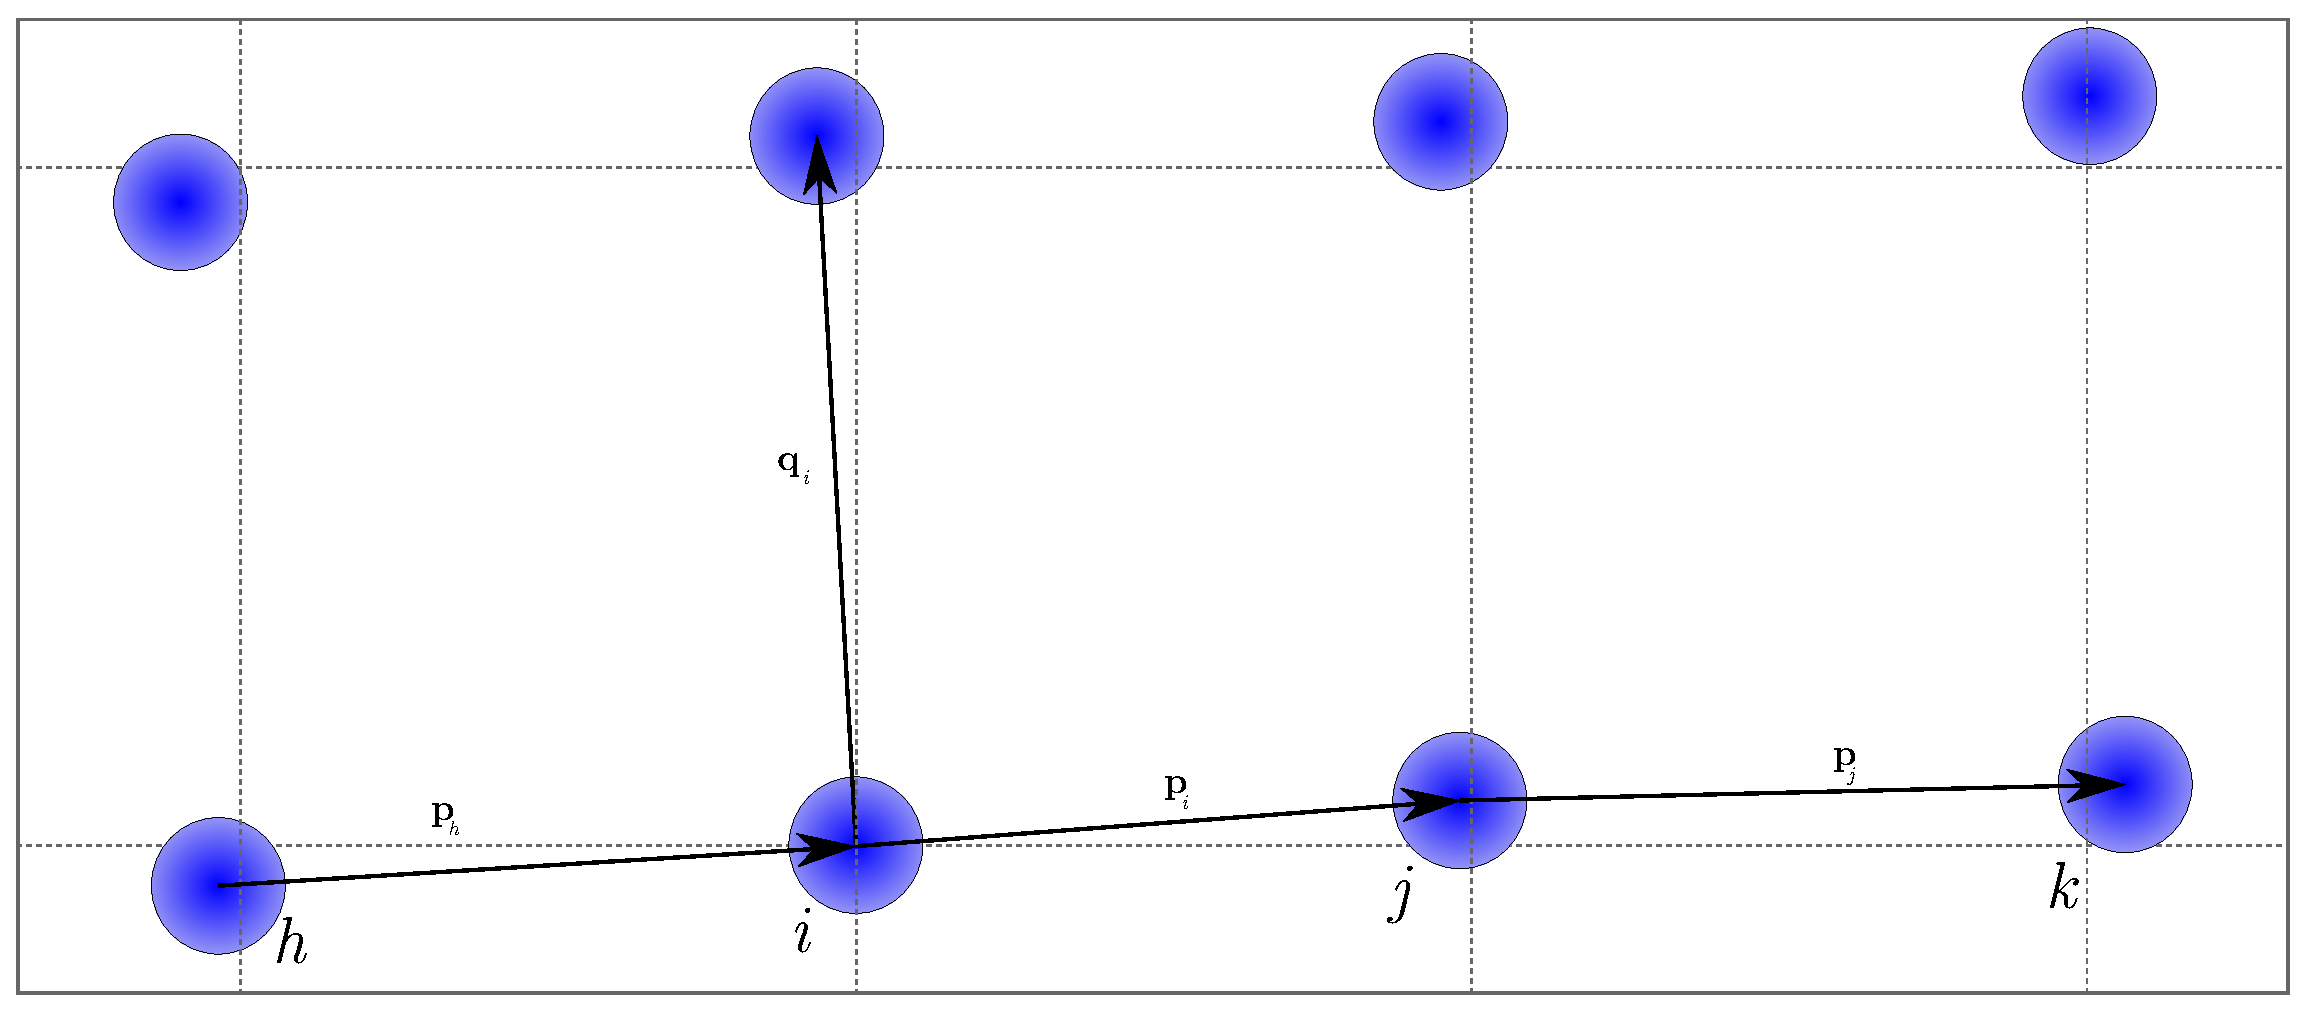
\includegraphics[width=\textwidth]{bonds}
\caption[Strained bonds in a dislocated crystal.]{The bonds that are considered for the $i$th atom in a region of crystal away from the slip plane; there is one bond to the nearest neighbour in the positive $x$~direction, $\mathbf{p}_i$, and one to the nearest neighbour in the positive $y$~direction, $\mathbf{q}_i$, to avoid double counting.\label{fig:bonds} }
\end{figure}





However there is a problem with this formulation. This assumes that every bond would, in equilibrium, be parallel to either the $x$ or the $y$ axis. This assumption is valid for the original Peierls model in which only displacements parallel to the $x$ direction were considered but the logarithmic term here represents a change in lattice orientation with position. A more nuanced approach requires some estimate of the local lattice orientation, if this is not done then the logarithmic term in \autoref{eqn:displacements} will mean that the strain in each bond will diverge, increasing with increasing distance from the dislocation core, whereas in reality the strains must be largest at the core.

There are clearly many possible ways of estimating the local lattice resistance, one possible method is to take the ideal orientation of the bond parallel to the slip plane for a particular bond to be paralell to the bonds on either side, i.e. as shown in \autoref{fig:bonds} the ideal orientation of $\mathbf{p}_i$ would be  parallel to $(\mathbf{p}_h + \mathbf{p}_j)$. The ideal orientation for $\mathbf{q}_i$ can be taken to be at \SI{90}{\degree} to this. So $\mathbf{\hat{i}}$ and $\mathbf{\hat{j}}$ in \autoref{eqn:estimate_strains} can be replaced with 
\begin{align}
\mathbf{\hat{i}}' &= \frac{(\mathbf{p}_h + \mathbf{p}_j)}{|\mathbf{p}_h + \mathbf{p}_j|} \nonumber \\
\mathbf{\hat{j}}' &= {\mathbf{\hat{i}}' \times \mathbf{\hat{k}}}
\end{align}
and the strain tensor can be calculated for each atom/unit cell, and hence the strain energy for each unit cell.



\FloatBarrier
\subsubsection{Misalignment energy}
\FloatBarrier
At the slip plane there is clearly going to be a break down of method highlighted above. For an atom immediately below the slip plane the identification of the nearest neighbour above the slip plane is perhaps not obvious. If the bond is taken to be simply  to the nearest atom above the slip plane ambiguities can arise 
It is possible that there will be two atoms equally close above the slip plane and such a simple criterion can lead to some atoms being bonded more than once and some atoms not being bonded. 

Instead a less arbitrary and more predictable method is to use the initial positions and assume that the $i$th atom can be bonded to two atoms in the layer above the slip plane. Since initially the horizontal spacing between atoms is $b$ for all atoms the two atoms must be within an interval $x_i^0 - b < x \leq x_i^0 + b$, as shown in \autoref{fig:slip_plane}. The energy for atom $i$ can be estimated from the average of the two bonds $\mathbf{q}_{i,\text{b}}$ and $\mathbf{q}_{i,\text{f}}$

\begin{figure}
\centering
\begin{subfigure}{\textwidth}
\centering
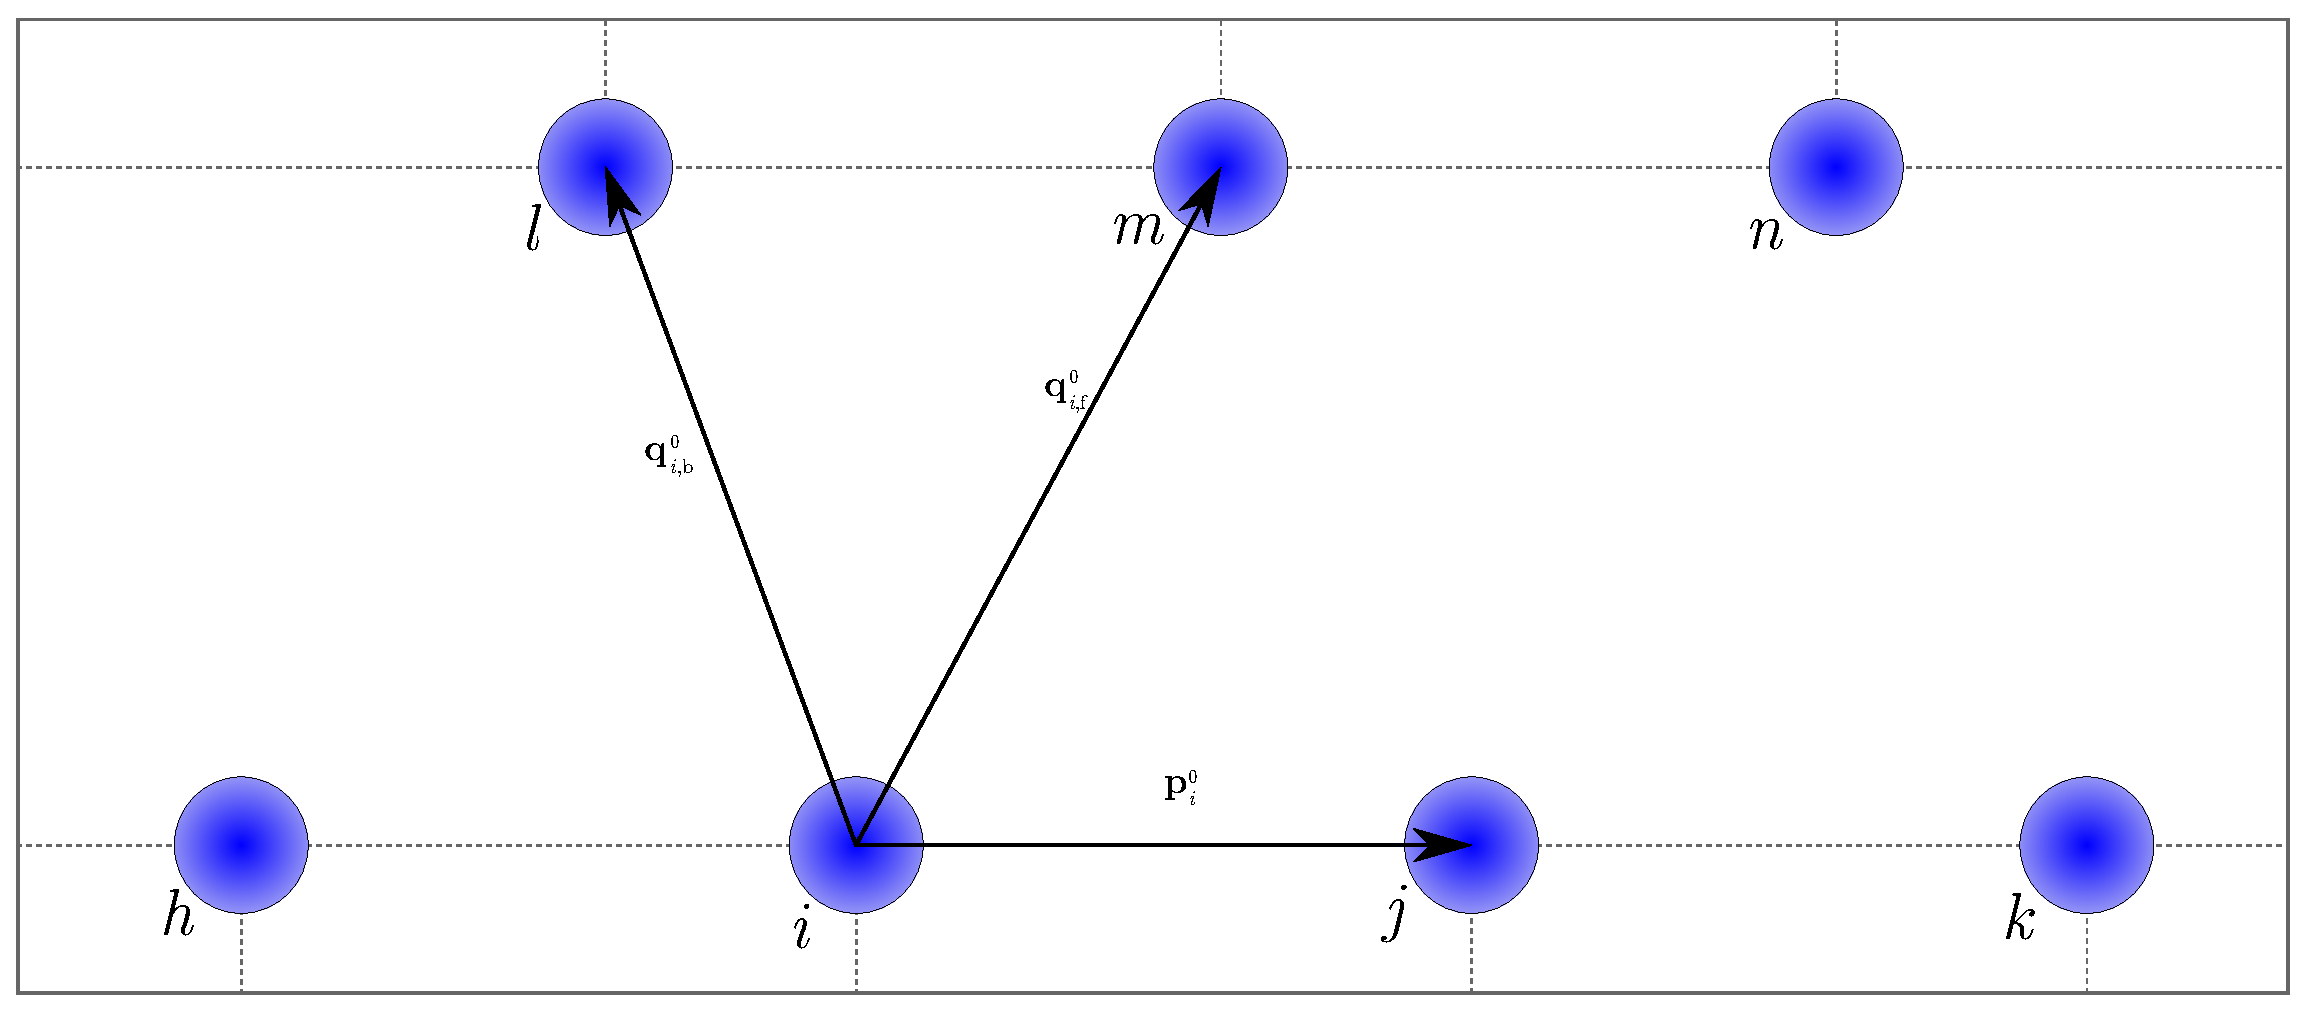
\includegraphics[width=\textwidth]{initial_slip_plane_bonds}
\caption{The initial positions of atoms either side of the slip plane.\label{fig:slip_plane_initial_positions}.}
\end{subfigure}
\par\medskip
\begin{subfigure}{\textwidth}
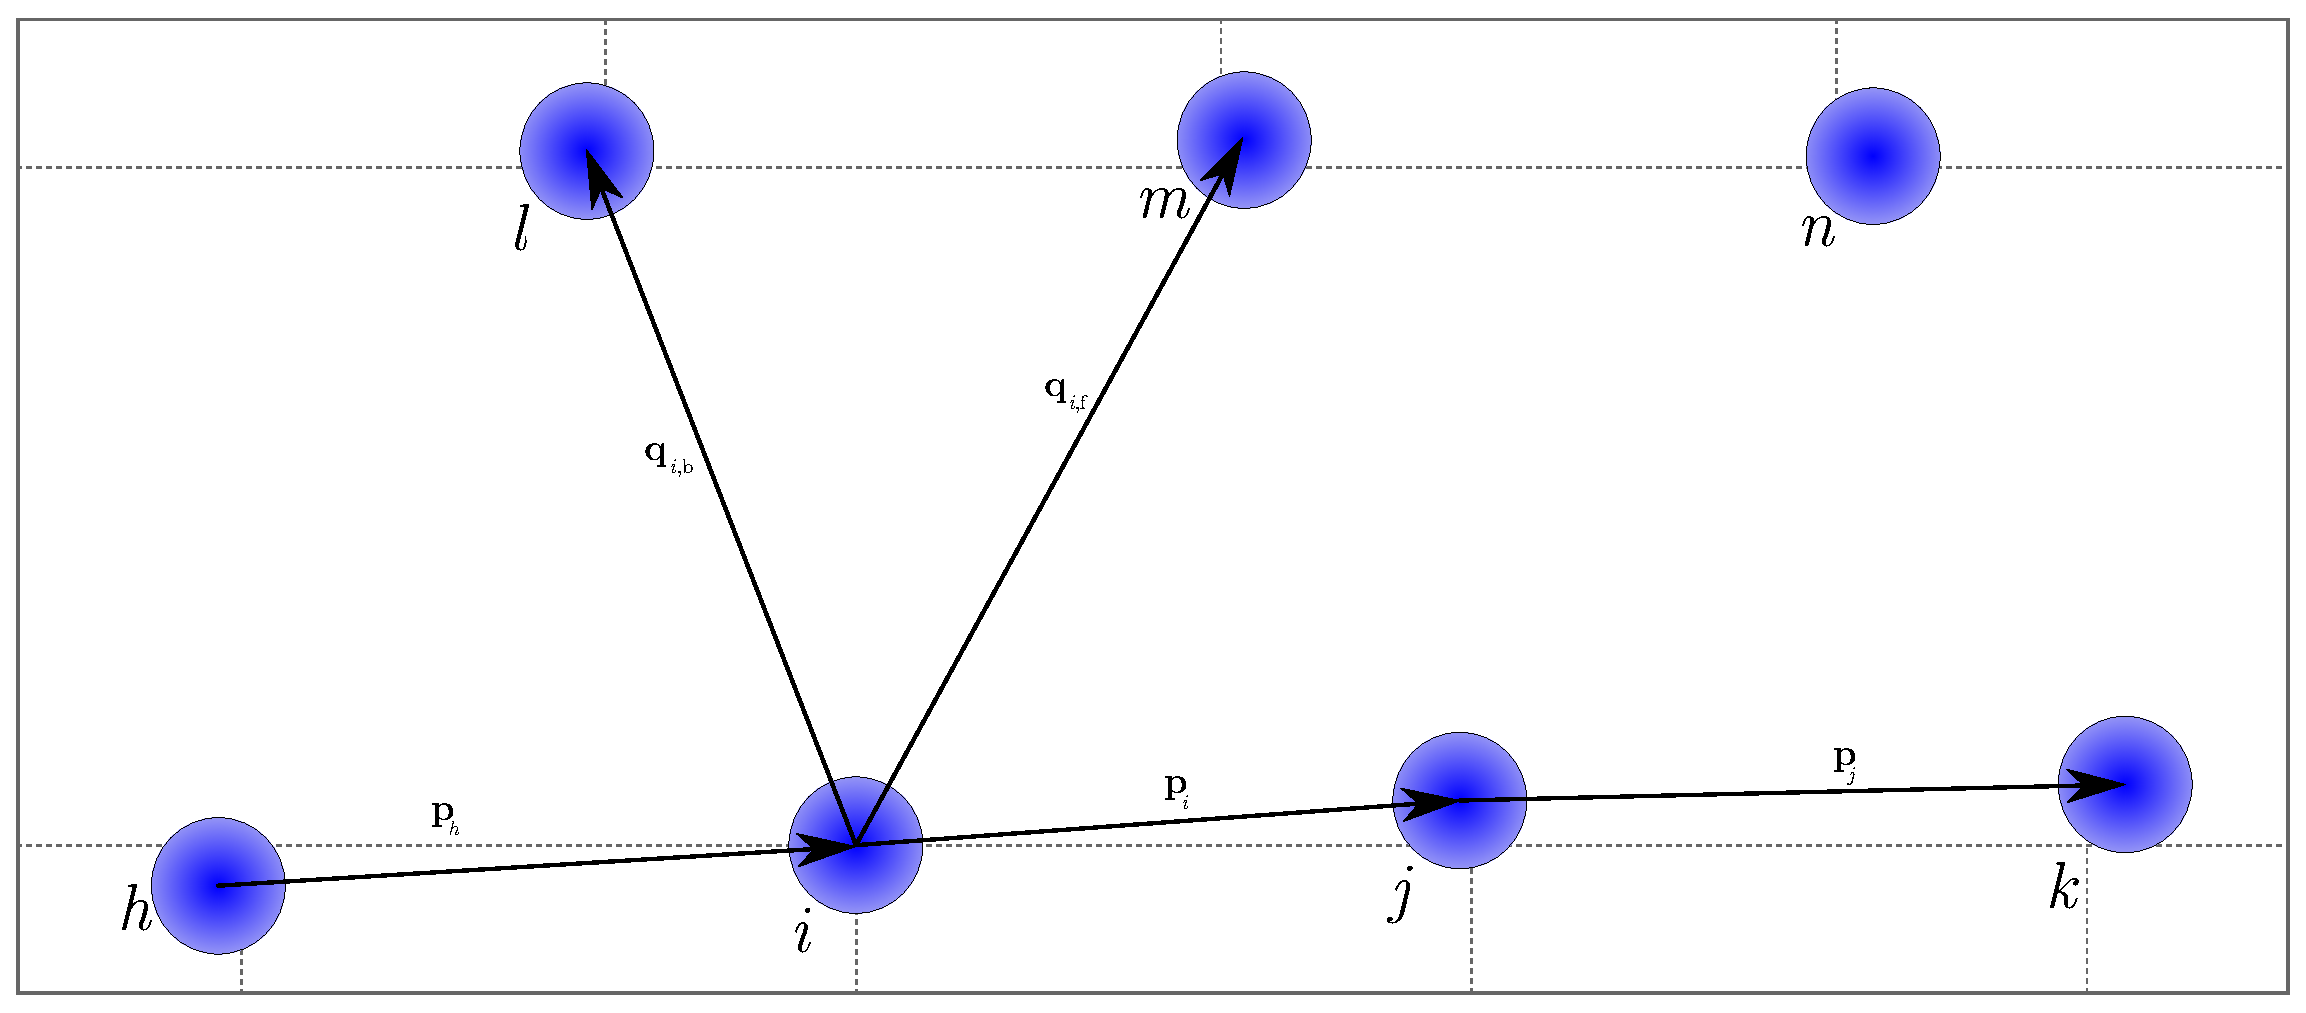
\includegraphics[width=\textwidth]{slip_plane_bonds}
\caption{The final positions of the atoms either side of the slip plane.\label{fig:slip_plane_final_positions}}
\end{subfigure}
\caption[Misaligned bonds cross the slip plane in a dislocated crystal.]{The slip plane before and after the application of the displacement field. The two atoms, $l$ and $m$, that can be considered bonded to the atom $i$ are shown along with the initial and final bonds, $\mathbf{q}_{i,\text{b}}$ and $\mathbf{q}_{i,\text{f}}$ which are backwards and forwards in the $x$ direction respectively. Also shown are the bonds $\mathbf{p}_h$ and $\mathbf{p}_j$ which are required to estimate the local orientation of the slip plane. \label{fig:slip_plane}}
\end{figure}


There are several methods to calculate the misaligned bonds. The simplest is to use the Frenkel approximation which, for an isotropic elastic material is 
\begin{equation}
U_i^\text{mis} = \frac{Gb^2}{4\pi^2} \left[\frac{d}{b}\right] \left[ 1 - \cos \left( \frac{2 \pi \phi}{d} \right) \right]
\end{equation}

which in terms of single crystal elastic constants takes $G=C_{66}$ (in Voigt notation see \cite{kelly_knowles2012chapter6_stress_strain}).

A more complete method for the calculation of the energy is to use the generalised stacking fault energy. Density functional theory can be used to calculate the energy of a stacking fault at an arbitrary misalignment. This is calculated by applying a displacement to two half crystals in a DFT simulation with periodic boundary conditions which introduces two opposing planar faults. The displacement is applied along the Burgers vector and the atoms are allowed to relax perpendicular to that displacement. Although the displacement field does not include any lateral (i.e. parallel to the lone vector) motion, allowing the DFT simulation of the stacking faults to relax laterally means that the energetic implications of lateral motion are included in the misalignment potential, although with an implicit assumption that the strains along the line vector do not extend beyond the slip plane. 

The energy changes with respect to a perfect crystal were considered and fitted with a simple empirical function:
\begin{equation}
\gamma(\phi) = \sum^{M}_{m=1} C_m \left[ 1 - \cos \left( \frac{2m\pi \phi}{b} \right) \right]
\end{equation}
where $\phi$ is the misalignment in the same units as the Burgers vector $b$, $m$ is an integer from \num{1} to $M$ and $C_m$ are coefficients fitted by a least-squares method to the energies calculated by DFT for different values of $\phi$. This is in units of \si{\joule\per\square\meter}, so a factor of $b$ must be applied to convert to a line energy in \si{\joule\per\meter}.


%%%%%%%%%%%%%%%%%%%%%%%%%%%%%%%%%%%%%%%%%%%%%%%%%%%%%%%%%%%%%%%5555%%%%%%%%%%%%%%%%%%%%%%%%%%%%%%%%%%%%%%%%%






%%%%%%%%%%%%%%%%%%%%%%%%%%%%%%%%%%%%%%%%%%%%%%%%%%%%%%%%%%%%%%%%%%%%%%%%%%%%%%%%%%%%%%%%%%%%%%%%%%%




\subsection{Empirical potentials}

Some materials can be described in a more physically insightful way than linear elasticity; as described in \autoref{sec:empirical_potentials}, empirical potentials have been developed for the field of molecular dynamics to be computationally convenient while at the same time approximating reality to a sufficient degree to gain insight into a system \cite{martinez2013}. One way to incorporate such potentials into the Peierls model described here is to write a simple python implementation of the potentials using the SciPy and NumPy packages and associated tools \cite{Numpy2011,Ipython2007,Millman2007,SciPy2001}; another way is to use the Atomic Simulation Environment \cite{ASE2017} or the python interface to the LAMMPS software package \cite{Plimpton1995,LAMMPS_web}.



To demonstrate the principle of using more physically informed potentials and hopefully capture more details of the energy changes as dislocations move the ionic solids were investigated using the Lennard-Jones potential:
\begin{equation}
\phi_{ij}(r_{ij}) = 4\epsilon_{ij} \left[ \left( \frac{\sigma_{ij}}{r_{ij}}\right)^{12}-     \left( \frac{\sigma_{ij}}{r_{ij}}\right)^6   \right]
\end{equation}
where $\epsilon_{ij}$ is the depth of the energy well and $\sigma_{ij}$ is the radius at which the energy is equal to zero or in the A--B form:
\begin{equation}
\phi_{ij}(r_{ij}) = \frac{A_{ij}}{r_{ij}^{12}} - \frac{B_{ij}}{r_{ij}^{6}}
\end{equation}
where $A_{ij} = 4\epsilon_{ij}\sigma_{ij}^{12}$ and $B_{ij} = 4 \epsilon_{ij} \sigma_{ij}^{6}$. The energy for any two atoms is then 
\begin{equation}
U_{ij}(r_{ij}) = \frac{1}{4\pi\epsilon_0} \frac{q_i q_j}{r_{ij}} + \frac{A_{ij}}{r_{ij}^{12}} - \frac{B_{ij}}{r_{ij}^{6}}
\end{equation}
where $\epsilon_0$ is the permittivity of free space.

The Lennard-Jones has been chosen as a simple example to demonstrate the application of empirical potentials for which fitted parameters are readily available \cite{Mao2014} and applicable to a class of materials for which the dislocation properties are not well explained by linear elasticity, the alkali halides.



\begin{table}
\centering
  \begin{tabular}{| m{3cm} | d{4} | d{-1} |}
  \hline
   Ion \rule{0pt}{3ex} & \multicolumn{1}{c|}{$\sigma_i$/\si{\angstrom}} & \multicolumn{1}{c|}{$\epsilon_i$/\si{\joule\per\mole}  }\\ \hline
   \ce{Li+} \rule{2ex}{0pt} & 1.715 & 241.25 \\
   \ce{Na+} & 2.497 & 327.44 \\
   \ce{K+} & 3.184 & 494.97 \\
   \ce{Rb+} & 3.302 & 1006.25 \\
   \ce{Cs+} & 3.440 & 2097.44 \\
   \ce{F-} & 3.954 & 27.05 \\
   \ce{Cl-} & 4.612 & 104.68 \\
   \ce{Br-} & 4.812 & 150.46  \\
   \ce{I-} & 5.197  & 176.56 \\
  \hline
  \end{tabular}
\caption[Lennard-Jones parameters.]{\rule[3ex]{0pt}{0pt} Parameters used for Lennard-Jones calculations from \cite{Mao2014}.\label{tab:LJ_params}}
\end{table}


The parameters used for the Lennard-Jones potential are shown in \autoref{tab:LJ_params}. They are calculated for each ion individually, to best reproduce lattice properties, and must be combined according to Lorentx-Berthelot rules:
\begin{align}
\epsilon_{ij} &= \sqrt[]{\epsilon_i \epsilon_j} \nonumber\\
\sigma_{ij} &= \frac{\sigma_i + \sigma_j}{2}
\end{align}

A na\"{\i}ve brute force implementation is given in Section~\ref{sec:ionic_energy_code} and an example input file is given for LAMMPS in Section~\ref{sec:lammps_input}. The LAMMPS pair style used was ``\texttt{lj/long/coul/long}'', the parameters for which are given in the example input file and is described in the LAMMPS documentation in \cite{LAMMPS_web}.




























































